%!TEX root = thesis.tex
\chapter{Methodology}
\label{ch:meth}


The network speed is always a bottleneck when transmitting complete CityJSON datasets over the web and doing something with the data, as the receiver can only do something with it once the data has arrived.
The assumption we thus make is that compressed datasets will have a better performance when the time that is gained in network transmission speed is larger than the time that is lost decoding the data after arrival.
This Chapter lays out the plan to benchmark the performance of several types of compressed CityJSON compared to uncompressed CityJSON, to find the advantages and disadvantage of techniques and give recommendations on what the best compression types would be given specific scenarios.

Shown in Figure~\ref{fig:workflow} is the structure of the methodology, divided into four general parts:
\begin{itemize}
\item The implementation of compression techniques for CityJSON
\item The preparation of datasets to test compression techniques with
\item Preparation of a testing platform that can work with both uncompressed and compressed CityJSON files
\item Testing and benchmarking the performance of different file types on the performance indicators of Table~\ref{tab:methindicators}, which were introduced in Section~\ref{sec:researchq}
\end{itemize}

The first three are finished prior to the benchmarking, in order to avoid having to redo work for part 2 when something had been changed in part 1.
The tasks in part 1 are grouped together because there is no necessary order and are implemented simultaneously.
All four are explained further in the next sections.

\begin{figure}[h!]
    \centering
    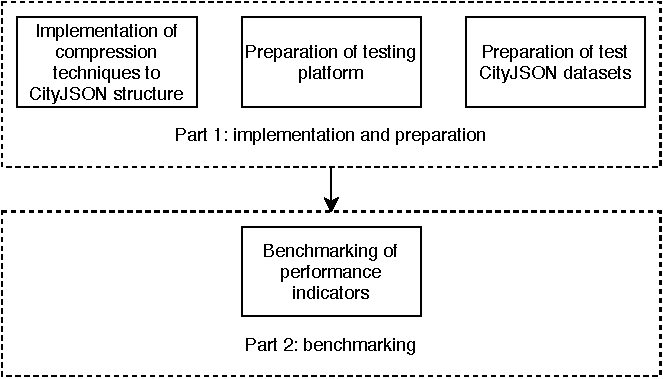
\includegraphics[scale=1]{figs/methodology/methodology_flow2.pdf}
    \caption{The general research workflow}
    \label{fig:workflow}
\end{figure}

\begin{table}[h!]
\begin{center}
 \begin{tabular}{ |c |} 
 \hline
  Compression type performance indicators \\ [0.5ex] 
 \hline\hline
 Visualisation time \\
 \hline
 Querying time \\
 \hline
 Spatial analysis time \\
 \hline
 Editing time \\
 \hline
 File size compression \\ 
 \hline
 Lossiness \\
 \hline
\end{tabular}
\caption{The six performance indicators on which variants of compressed CityJSON are assessed}
\label{tab:methindicators}
\end{center}
\end{table}




\section{Implementation of compression techniques}
\label{sec:compressionimplementation}

In Chapter~\ref{ch:theory} a multitude of compression techniques has been introduced.
Different combinations of these techniques are applied to the CityJSON structure and be compared on the six defined performance indicators (see Table~\ref{tab:methindicators}), with the performance of uncompressed CityJSON as the baseline.
A possible outcome is that certain combinations of techniques are more suitable for specific purposes, making it difficult to choose one that is the best.
Chapter~\ref{ch:bmresults} shows which compression types 
For this reason, there is a depthly discussion about it in Chapter~\ref{ch:bmresults}.

Table~\ref{tab:compressionmethods} shows which combinations of compression techniques I implement on CityJSON and benchmark on time performance.
The table has a divide between compression methods where the geometries are kept as is, and where they have been replaced by Draco-compressed geometry.
All other names besides "original" and "draco" indicate either the inclusion of a binary format or a compression technique.

The only compression technique that has not been explained in Chapter~\ref{ch:theory} is the so-called replace technique, which I have created.
It means that all keys and values of "CityObjects" from the \ac{json} structure are copied to a separate array.
The elements of the array are sorted by frequency, and the keys and values in the \ac{json} are replaced with a reference to the array.
This has three supposed advantages: 

\begin{enumerate}
\item The \ac{json} structure is retained, of which parts could be reconstituted as wanted. It would for instance be possible to only decode the first City Object rather than all of them. When using a compression technique directly on the \ac{json} structure, all data has to be decoded prior to use.
\item The array allows for greater compression as the keys and values can be compressed at once with for example zlib, as opposed to compressing all of them individually.
\item Redundancy is removed, as keys and values that appear more than once are only stored as one array element.
\end{enumerate}
The array can be stored as a member of the CityJSON object and thus optionally be included in a \ac{cbor} representation.
An example of how a dataset compressed in this way looks like is found in Section~\ref{sec:implreplace}.


Ultimately there are 20 different types of CityJSON tested, of which 19 are compressed variants and 1 is original CityJSON.
However, "original CityJSON" is defined as including the "transform" member (as stated in Section~\ref{sec:researchq}, with "transform" being explained in Section~\ref{sec:cityjsonexplained}), which is done for the uniformity of datasets and because Draco needs coordinates to be stored in this manner before compression.
It is however already a form of compression, but included in the CityJSON specification \citep{cityjsonspecs}.



They tested CityJSON types are divided into two categories: having geometry compressed by Draco, or geometry as originally implemented in CityJSON.
So there are actually 10 pairs, within which the difference is the use of Draco.
Table~\ref{tab:compressionmethods} shows all CityJSON implementations, and in the following enumeration a brief description is given for all 10 combinations:

\begin{enumerate}
\item The dataset is in the style of regular CityJSON, but needs to include "transform". "original" is the baseline to which all other combinations are compared. 
As for "draco", the Draco \ac{blob} is placed underneath the \ac{json} structure, with a delimiter inbetween. 
It can not be added as a member of the CityJSON object as \ac{json} does not allow binary values.
This means that the result is a binary file.
\item The same as 1, but with the complete file compressed with zlib (see Section~\ref{sec:zlib}).
\item Similar to 1, but with the CityJSON object parsed into \ac{cbor} (see Section~\ref{sec:cbor}). 
In this case, the Draco \ac{blob} is added as a member of the CityJSON object as it does allow for binary values.
This would make it easier and quicker to read as well, since the file does not need to be split by a delimiter.
\item Encoded in \ac{cbor} like 3, but all keys and string values of the CityJSON object are compressed by smaz.
This only works in combination with cbor, because strings are binary-encoded by smaz.
\item Same as 3, but with the resulting \ac{cbor} (Section~\ref{sec:cbor}) compressed with zlib (Subsection~\ref{sec:zlib}).
\item Similar to 1, but with all keys and values copied to an array and replaced by references.
\item Same as 6, but with the array  compressed with zlib.
\item Same as 6, but with the CityJSON object parsed into \ac{cbor}.
\item Same as 8, but with the array compresed with zlib.
\item Same as 8, but with the array compressed with Huffman coding (see Section~\ref{sec:huffman}).
\end{enumerate}


%For compression combinations using Draco, the array of vertices and all the boundaries of Geometry Objects are stripped from the dataset.
%The geometries are compressed by Draco and stored in the file as a \ac{blob}.


\begin{table}[]
\begin{tabular}{|l||l|l|}
\hline
 & \textbf{Original geometry}    & \textbf{Draco geometry}    \\
\hline \hline
1 & original                      & draco                      \\
\hline
2 & original-zlib                 & draco-zlib                 \\
\hline
3 &original-cbor                 & draco-cbor                 \\
\hline
4 & original-cbor-zlib            & draco-cbor-zlib            \\
\hline
5 & original-cbor-smaz            & draco-cbor-smaz            \\
\hline
6 & original-replace              & draco-replace              \\
\hline
7 & original-replace-zlib         & draco-replace-zlib         \\
\hline
8 & original-cbor-replace         & draco-cbor-replace         \\
\hline
9 & original-cbor-replace-zlib    & draco-cbor-replace-zlib    \\
\hline
10 & original-cbor-replace-huffman & draco-cbor-replace-huffman \\
\hline
\end{tabular}
\caption{Combinations of compression methods, separated by type of geometry.}
\label{tab:compressionmethods}
\end{table}



Decompression functions have to be written as well, both to be able to assess the loss of information due to the compression process and to allow for the data to be decompressed for use in the web application.
Loss that is expected to see mainly concerns the precision (or even accuracy) of coordinates, the ordering of vertices, and the ordering of City Objects.
The former is a large problem as the thesis concerns geographical data that can be used for analysis, as opposed to visualisation only.
It can happen when Draco is not used in the correct way (see Section~\ref{rwdraco}).
The second one can happen with Draco as well, but since its geometries are triangulated it only means that vertices of triangles are ordered differently which is not problematic.
Lastly, a different ordering of City Objects is acceptable because all information is retained, but it should still be noted as it is possible that a dataset is ordered with a purpose.



Encoding \ac{json} into \ac{cbor} is likely to give a better performance than other compression methods (such as directly compressing the datasets with zlib), as explained by \citet{UBJSON2020}.
While zlib should decrease the file sizes further than \ac{cbor}, the processing---encoding and decoding---of zlib-compressed data is less efficient.
In addition, a binary \ac{json}-like format enables a person to still inspect human readable parts (such as strings), which can help with debugging.
Another option however is to zlib a \ac{cbor} file, which can be done if storage space is an important issue.

A possibility is to create an original binary format for CityJSON.
However, since \ac{json} can already be directly encoded into \ac{cbor}, this is not necessary as it would overcomplicate it.
It could be done in a similar way as b3dm (see Section~\ref{sec:b3dm}) by retaining the \ac{json} structure and having a separate part for binary values.
However, in this way only values are stored in binary and not keys, and when creating a dataset it needs to be chosen which values are stored in binary.

%\section{Benchmarking and comparison of results}
\section{Performance of (compressed) datasets}
\label{sec:methperformance}
The performance of the different compression method combinations are assessed following the six main performance indicators from Table~\ref{tab:methindicators}.
For each of these, specific data operations are defined that are tested, with original CityJSON datasets as the baseline to which the performance of compressed CityJSON files is compared.
Below follows an explanation on all operations, and an overview can be seen on Figure~\ref{fig:benchmarking}.

The file size performance is defined as the compression factor.
This is the size of a compressed dataset divided by the size of the uncompressed one.
For all other operations, the performance is defined as the time that it takes to complete the operation with the compressed dataset divided by the time that it takes to finish the same operation with the original dataset.

\begin{enumerate}
\item Querying. Querying one City Object of a dataset (by its ID) and querying all City Objects (by an attribute field that all City Objects have in common). The query returns the matching City Objects including the vertices that their Geometry Objects refer to.
\item Visualisation. The rendering of all City Objects of a dataset.
\item Spatial analysis. Buffering one City Object and buffering all City Objects by 1 metre in 2D, so their geometries are first projected to 2D.
\item Editing of attributes. Adding "1" at the end of the ID of one City Object, and doing the same thing for all City Objects. If the file had to be decompressed before the operation, it has to be compressed again.
\item Editing of geometry. Raising the height of all vertices of one City Object by 1 metre, and doing the same thing for all objects. If the file had to be decompressed before the operation, it has to be compressed again.
\end{enumerate}


These are performed with all datasets, which are compressed as described in Section~\ref{sec:compressionimplementation}.
All combinations of operations, datasets, and compressions are thus assessed.
The assessment is done by benchmarking the time that is needed to complete an operation, taken as the average over ten attempts to eliminate abnormalities.


Being secondary indicators, lossiness and possibility of asynchronous loading are described separately.
The former can involve loss of object order, loss of vertex order, and triangulation of a file that was originally non-triangulated

Ultimately, by putting all results in a table, the best (combination of) methods can be found for every separate criterion.
On each of the indicators, the compression method is evaluated and ranked.
An overview of the benchmarking workflow can be found on Figure~\ref{fig:benchmarking}.


\section{Testing platform and benchmarking}
\label{methtestingplatform}

To test the performance of using CityJSON and its different compressed variants on the web, a web application has to be set up that enables this.
While two options already exist (\citet{Boersma2019} and \citet{CityJSON2020}), it is better to create one that is of a simple structure so that it can easily be adapted for experimental functionalities for the research.

Therefore, I have set up a Flask application which acts like a server, which integrates functionalities of Draco \citep{dracoperformance}, cjio \citep{cjio}, self-created functions, and harp.gl \citep{harpgl} through JavaScript.
An explanation of the mentioned tools is given in Chapter \ref{ch:tools}.
The platform enables to do the operations of Figure~\ref{tab:compressionmethods} on all (compressed) CityJSON variants by visiting corresponding Flask routes in a browser.
The operations have short names as shown in Table~\ref{tab:operationnames} to easily identify them in the results.


Every dataset (8 of them, having different characteristics---see Section~\ref{methdataset}) is compressed by every CityJSON implementation type (20) and then benchmarked on the time that it takes to complete every individual operation (9) on them.
This means that there are 1440 planned resulting time benchmarks.
Every time benchmark is performed multiple times in order to retrieve more accurate results, as there are some uncertainties in the timing meaning that every iteration will have a slightly different time value.
The time values are in milliseconds and outliers within the 10 iterations are removed based on having a z-score of 2.
The z-score is the amount of standard deviations that a measurement differs from the average of the set.

The benchmarks are performed through a web testing library that visits the specific Flask route for a combination of dataset, operation, and compression type in a browser with a throttled network speed to simulate practical conditions.

\begin{table}[h!]
\begin{tabular}{|c|c|}
    \hline
    Visualisation&visualise\\
    &\\
    \hline
    \multirow{2}{*}{Querying}&queryone\\
    &queryall\\
    \hline
    \multirow{2}{*}{Spatial analysis}&bufferone\\
    &bufferall\\
    \hline
    \multirow{2}{*}{Editing (attributes)}&editattrone\\
    &editattrall\\
    \hline
    \multirow{2}{*}{Editing (geom)}&editgeomone\\
    &editgeomall\\
\hline
\end{tabular}
\caption{Names for all operations in the results.}
\label{tab:operationnames}
\end{table}



\begin{landscape}\centering
\thispagestyle{empty} % removes page number
\begin{figure}[htbp]
%\advance\leftskip-5cm

    \hspace*{-2.8cm}  
    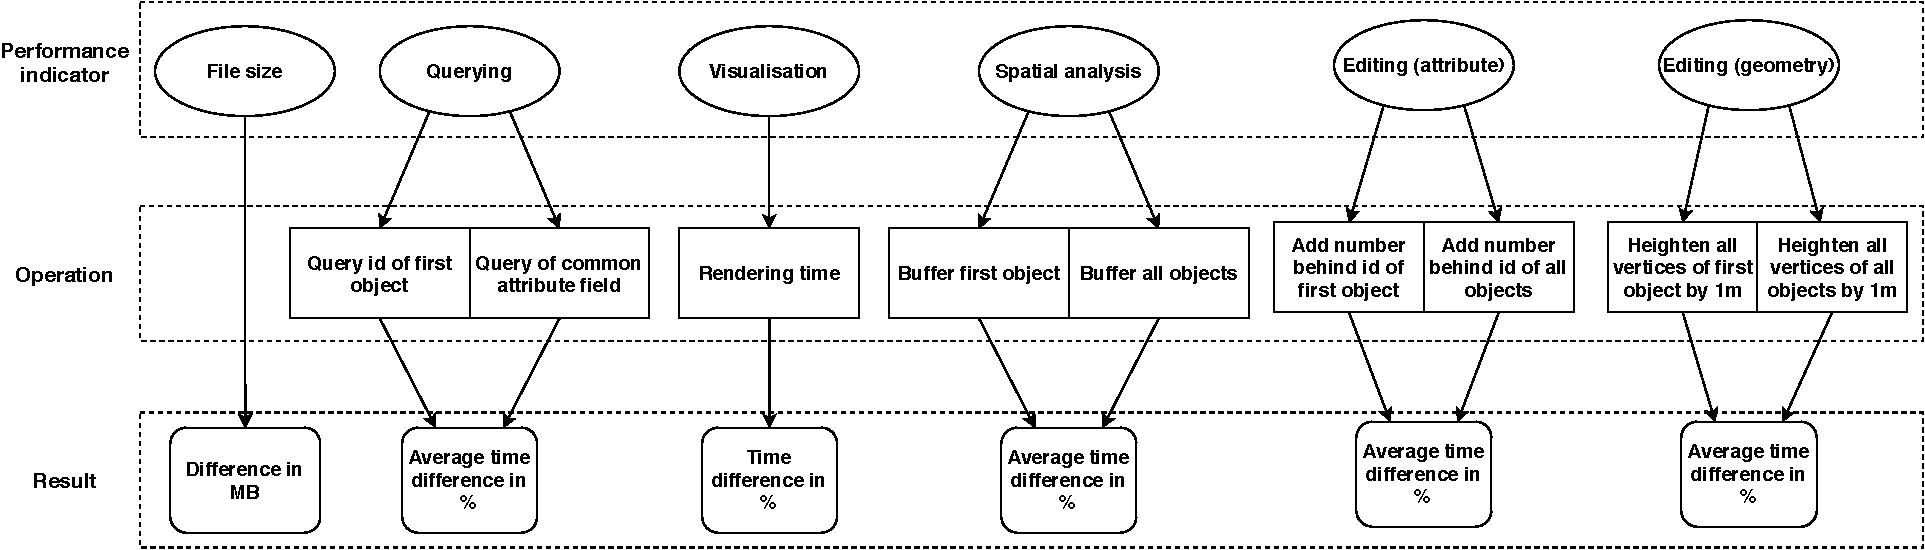
\includegraphics[scale=0.83]{figs/methodology/benchmarking.pdf}
    \caption{The workflow of the benchmarking. This is done for every compression method and all datasets.}
    \label{fig:benchmarking}
\end{figure}
\end{landscape}


\section{Dataset preparation}
\label{methdataset}

Since different dataset characteristics can influence the compression factor and benchmarking performance of compression types, it would be good to use a varied selection of CityJSON datasets to test with.
For example, a compression method that makes use of the repetition of data will work better when there are more repeated elements in the dataset that can be taken advantage of.
The file size of the to be compressed dataset can be an indication of this, as larger files tend to have more repeated parts. 
For example the keys \texttt{"type"} and \texttt{"boundaries"} are there for every City Object, and possibly repeated attributes.
For this reason it is expected that larger datasets will generally have a lower file size multiplier.

The LOD is interesting because it indicates a difference in the geometrical complexity of the features.
It is possible that there is a difference to be seen in the impact of Draco compression depending on it.
The variety of feature types is another characteristic because similarly to LOD, terrains can potentially have more complex geometries than buildings.
As for attributes, the amount of them per feature could impact the performance of attribute compression, as it would be expected that more attributes are percentually compressed further.
Lastly, the language they are in can potentially make a difference when the smaz compression technique is used.

The file size will however be the most important about datasets, since the bottleneck is assumed to be the network speed when using large datasets on the web.
If a dataset is already small, for example 1 MB, compressing it to 0.7 MB would only have the file be downloaded 0.06 seconds faster on a 5 MB/s (or 40 Mbit/s) internet connection (which is the average in The Netherlands \.
Compressing a 100 MB file to 70 MB on the other hand will improve the transmission speed by 6 seconds.

An overview of important dataset characteristics can be seen below, and the chosen datasets can be found in Section \ref{datasetdescription}.

\begin{itemize}
\item{File size}
\item{Repetition of data}
\item{LOD}
\item{Variety of feature types}
\item{Size of attributes}
\item{Attribute language}
\end{itemize}

\section{Overview}
Concludingly, the following results are presented in Chapter~\ref{ch:bmresults}:
\begin{enumerate}
\item The resulting compression factors of individual datasets as compressed by every compression type, and the average compression factor per compression type.
\item The encoding time of individual datasets with every compression type, and the average encoding time per compression type.
\item Time performance benchmarks on all compression type, dataset, and operation combinations with both server implementations. As conclusion, plots are made showing the average performance of a compression type per individual dataset, meaning that the operations are averaged. With this you can answer the question: "I have this dataset and want to do anything with it, which compression types are the most suitable?". Taking averages over all datasets is not done since they are not a representative selection, as opposed to the operations.
\end{enumerate}



